% WatchGate — presentación de kickoff
% Compilar con: xelatex main.tex  (dos pasadas para el índice/enlaces)
\documentclass[9pt,aspectratio=169]{beamer}

\usepackage{fontspec}
\usepackage[table]{xcolor}
\usepackage{tikz}
\usetikzlibrary{positioning,arrows.meta,shapes.geometric,calc,backgrounds,fit}
\usepackage{graphicx}
\usepackage{booktabs}
\usepackage{pifont}
\usepackage{microtype}
\usepackage{hyperref}
\hypersetup{colorlinks=true, linkcolor=brandcyan, urlcolor=brandcyan, pdftitle={WatchGate}, pdfauthor={Equipo WatchGate}}

% ---------- tipografía ----------
% Optima: titulares (grave, algo monumental -- un "sello" de vigilancia).
% Charter: cuerpo de texto (serif cálida, muy legible).
% Menlo: código, diffs, datos.
\setmainfont{Charter}
\newfontfamily\OptimaFont{Optima}
\newfontfamily\OptimaFontBold{Optima}[BoldFont={Optima Bold}]
\newfontfamily\MenloFont{Menlo}

% ---------- paleta (extraída del logo real de la UMA y de la memoria) ----------
\definecolor{brandnavy}{HTML}{002959}
\definecolor{brandnavy2}{HTML}{123A66}
\definecolor{brandcyan}{HTML}{00ADCB}
\definecolor{paper}{HTML}{F5F6F8}
\definecolor{paperraised}{HTML}{FFFFFF}
\definecolor{ink}{HTML}{14202E}
\definecolor{inksoft}{HTML}{4B586A}
\definecolor{linecol}{HTML}{D6DCE5}
\definecolor{linestrong}{HTML}{AAB8CA}
\definecolor{semred}{HTML}{B23A2E}
\definecolor{semredsoft}{HTML}{F3E1DF}
\definecolor{samber}{HTML}{9C6B0C}
\definecolor{sambersoft}{HTML}{F1E6CE}
\definecolor{semgreen}{HTML}{2E7D4F}
\definecolor{semgreensoft}{HTML}{DCEBE1}
\definecolor{boxfill}{HTML}{E7EEF6}

% ---------- limpieza del tema base ----------
\usetheme{default}
\setbeamertemplate{navigation symbols}{}
\beamertemplatenavigationsymbolsempty
\setbeamercolor{background canvas}{bg=paper}
\setbeamercolor{normal text}{fg=ink,bg=paper}
\setbeamercolor{structure}{fg=brandnavy2}
\setbeamercolor{itemize item}{fg=brandcyan}
\setbeamercolor{itemize subitem}{fg=inksoft}
\setbeamertemplate{itemize item}{\textcolor{brandcyan}{\rule{5.5pt}{2pt}}}
\setbeamertemplate{itemize subitem}{\textcolor{linestrong}{\rule{4pt}{1.4pt}}}
\setbeamerfont{itemize/enumerate body}{size=\normalsize}
\setlength{\leftmargini}{16pt}
\setbeamertemplate{itemize items}[default]

% título de cada slide: etiqueta pequeña versalita + regla cian (como en la memoria)
\setbeamertemplate{frametitle}{%
  \vspace{6pt}%
  {\OptimaFontBold\bfseries\fontsize{16}{18}\selectfont\color{brandnavy}\MakeUppercase{\insertframetitle}}\\[3pt]
  {\color{brandcyan}\rule{\textwidth}{1.1pt}}%
  \vspace{2pt}%
}

% pie de página discreto
\setbeamertemplate{footline}{%
  \hbox{%
    \begin{beamercolorbox}[wd=\paperwidth,ht=2.6ex,dp=1.4ex,leftskip=14pt,rightskip=14pt]{footline}
      {\MenloFont\fontsize{6.6}{7}\selectfont\color{inksoft}%
       WATCHGATE\hfill Cátedra de Ciberseguridad \textperiodcentered\ UMA \textperiodcentered\ 2026\hfill\insertframenumber/\inserttotalframenumber}
    \end{beamercolorbox}%
  }%
}
\setbeamertemplate{headline}{}
\setbeamercolor{footline}{bg=paper,fg=inksoft}

% ---------- estilos TikZ reutilizables ----------
% Estilo "diagrama de ingeniería": esquinas rectas, relleno azul pálido,
% borde marino fino -- el mismo lenguaje visual que la Figura 1 de la memoria.
\tikzset{
  card/.style={draw=brandnavy2, line width=0.6pt, fill=boxfill, align=left, inner sep=8pt},
  cardcyan/.style={card},
  arrow/.style={-{Stealth[length=5pt,width=4pt]}, brandnavy2, line width=0.9pt},
  thinarrow/.style={-{Stealth[length=4pt,width=3.4pt]}, brandnavy2, line width=0.7pt},
  dotarrow/.style={-{Stealth[length=4.5pt,width=3.6pt]}, inksoft, line width=0.7pt, dash pattern=on 2.6pt off 2.2pt},
}

% \lbl y \sub son declaraciones de formato (como \bfseries), no macros con
% argumento: se usan como {\lbl Texto...}, siempre dentro de un grupo.
\newcommand{\lbl}{\OptimaFontBold\bfseries\fontsize{8.6}{9.5}\selectfont\color{brandnavy2}}
\newcommand{\sub}{\fontsize{7.6}{9}\selectfont\color{inksoft}}

\title{WatchGate}
\author{Equipo WatchGate}
\date{}

\begin{document}

% ======================================================================
% Portada con foto (versión que prefiere el equipo).
\begin{frame}[plain]
\begin{tikzpicture}[remember picture, overlay]
  \node[anchor=south west, inner sep=0] at (current page.south west)
    {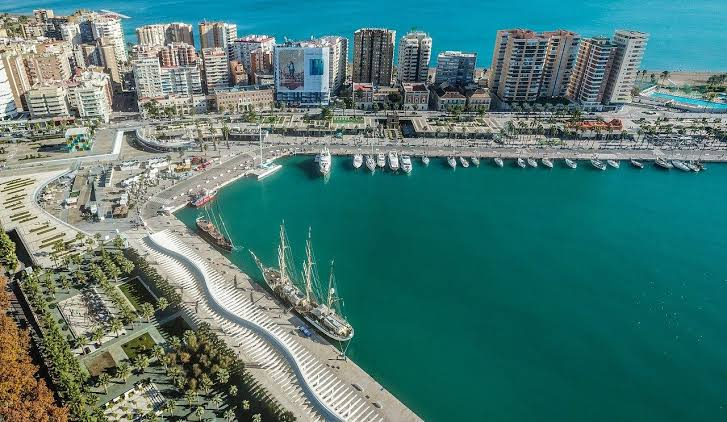
\includegraphics[width=\paperwidth,height=\paperheight,keepaspectratio=false]{malaga.jpeg}};
  \fill[brandnavy, opacity=0.62] (current page.south west) rectangle (current page.north east);
\end{tikzpicture}
\begin{tikzpicture}[remember picture, overlay, x=1cm, y=1cm]
  \node[anchor=south west, text=paperraised, inner sep=0] at ($(current page.south west)+(1.1,1.05)$)
    {\begin{minipage}{9.2cm}
      {\OptimaFontBold\bfseries\fontsize{18}{18}\selectfont\color{brandcyan}\MakeUppercase{Cátedra de Ciberseguridad \textperiodcentered\ Universidad de Málaga}}\\[14pt]
      {\OptimaFontBold\bfseries\fontsize{52}{52}\selectfont\color{paperraised}Watch\textcolor{brandcyan}{Gate}}\\[10pt]
      {\fontsize{13.5}{16}\selectfont\color{paperraised} Sistema de \emph{scoring} de riesgo para la revisión\\automatizada de \emph{pull requests} en pipelines CI/CD}\\[13pt]
      {\fontsize{9}{11}\selectfont Javier Martín Jurado \textperiodcentered\ Pablo Jiménez Castro \textperiodcentered\ Pablo Ayllón García\\[3pt] Málaga, julio de 2026}
    \end{minipage}};
  \node[anchor=south east, fill=paperraised, rounded corners=3pt, inner sep=6pt] at ($(current page.south east)+(-1.0,0.9)$)
    {
\includegraphics[height=0.55cm]{logos/uma.png}};
\end{tikzpicture}
\end{frame}

% ======================================================================
\begin{frame}{Índice}
\begin{columns}[T]
\begin{column}{0.5\textwidth}
\begin{itemize}
  \setlength\itemsep{10pt}
  \item[\textcolor{brandcyan}{\OptimaFontBold 01}] El problema
  \item[\textcolor{brandcyan}{\OptimaFontBold 02}] Estado del arte
  \item[\textcolor{brandcyan}{\OptimaFontBold 03}] Arquitectura
  \item[\textcolor{brandcyan}{\OptimaFontBold 04}] El contrato entre capas
  \item[\textcolor{brandcyan}{\OptimaFontBold 05}] Las cuatro capas
  \item[\textcolor{brandcyan}{\OptimaFontBold 06}] Formato de salida
\end{itemize}
\end{column}
\begin{column}{0.5\textwidth}
\begin{itemize}
  \setlength\itemsep{10pt}
  \item[\textcolor{brandcyan}{\OptimaFontBold 07}] Capa estática
  \item[\textcolor{brandcyan}{\OptimaFontBold 08}] Capa de dependencias
  \item[\textcolor{brandcyan}{\OptimaFontBold 09}] Capa de reputación
  \item[\textcolor{brandcyan}{\OptimaFontBold 10}] Capa semántica
  \item[\textcolor{brandcyan}{\OptimaFontBold 11}] Infraestructura necesaria
\end{itemize}
\end{column}
\end{columns}
\end{frame}

% ======================================================================
\begin{frame}{01 \textperiodcentered\ El problema}
\noindent{\large La revisión humana, como única barrera, tiene limitaciones estructurales}\par\vspace{6pt}
{\color{inksoft}\small Fatiga del revisor, sesgo de confianza hacia colaboradores habituales, y la dificultad de detectar intención maliciosa cuando se disimula dentro de un cambio que parece legítimo. No es hipotético: son tres campañas reales de los últimos dos años.}

\vspace{10pt}
\begin{columns}[T,onlytextwidth]
\begin{column}{0.333\textwidth}
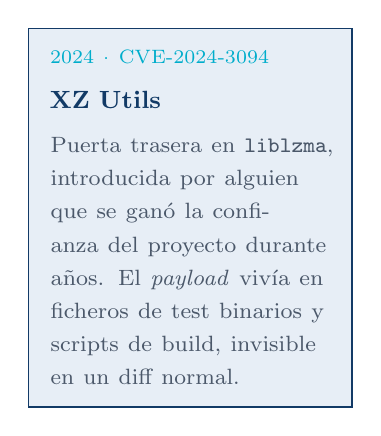
\begin{tikzpicture}
\node[card, text width=3.55cm, minimum height=3.35cm] (a) {
  {\MenloFont\fontsize{6.6}{7}\selectfont\color{brandcyan} 2024 \textperiodcentered\ CVE-2024-3094}\\[4pt]
  {\lbl XZ Utils}\\[4pt]
  {\sub Puerta trasera en \texttt{liblzma}, introducida por alguien que se ganó la confianza del proyecto durante años. El \emph{payload} vivía en ficheros de test binarios y scripts de build, invisible en un diff normal.}
};
\end{tikzpicture}
\end{column}
\begin{column}{0.333\textwidth}
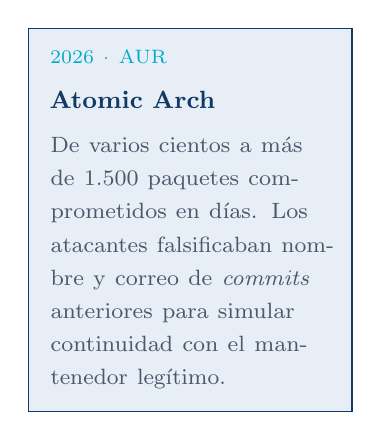
\begin{tikzpicture}
\node[card, text width=3.55cm, minimum height=3.35cm] (b) {
  {\MenloFont\fontsize{6.6}{7}\selectfont\color{brandcyan} 2026 \textperiodcentered\ AUR}\\[4pt]
  {\lbl Atomic Arch}\\[4pt]
  {\sub De varios cientos a más de 1.500 paquetes comprometidos en días. Los atacantes falsificaban nombre y correo de \emph{commits} anteriores para simular continuidad con el mantenedor legítimo.}
};
\end{tikzpicture}
\end{column}
\begin{column}{0.333\textwidth}
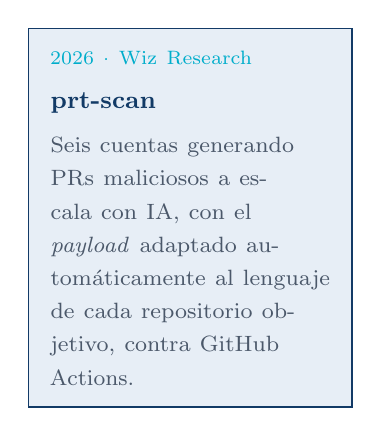
\begin{tikzpicture}
\node[card, text width=3.55cm, minimum height=3.35cm] (c) {
  {\MenloFont\fontsize{6.6}{7}\selectfont\color{brandcyan} 2026 \textperiodcentered\ Wiz Research}\\[4pt]
  {\lbl prt-scan}\\[4pt]
  {\sub Seis cuentas generando PRs maliciosos a escala con IA, con el \emph{payload} adaptado automáticamente al lenguaje de cada repositorio objetivo, contra GitHub Actions.}
};
\end{tikzpicture}
\end{column}
\end{columns}
\end{frame}

% ======================================================================
\begin{frame}{02 \textperiodcentered\ Estado del arte}
\noindent{\large Las herramientas existentes cubren una única capa del problema}\par\vspace{8pt}
{\color{inksoft}\small Socket.dev y GuardDog miran la dependencia externa, no el código del PR. BewAIre (Datadog) razona sobre el diff con LLM, pero es interna y cerrada. Ninguna cruza identidad declarada contra historial real, ni documenta cómo gobierna su propia IA.}

\vspace{12pt}
\centering
\renewcommand{\arraystretch}{1.35}
{\small
\begin{tabular}{@{}l ccccc@{}}
\toprule
\textbf{\footnotesize Herramienta} & \textbf{\footnotesize Abierta} & \textbf{\footnotesize Multiplat.} & \textbf{\footnotesize Identidad vs.\ hist.} & \textbf{\footnotesize Explicable} & \textbf{\footnotesize Gobierna LLM} \\
\midrule
Socket.dev / GuardDog & $\sim^{1}$ & \ding{55} & \ding{55} & $\sim^{2}$ & n/a \\
BewAIre \emph{(Datadog, interno)} & \ding{55} & \ding{55} & \ding{55} & \ding{55}$^{3}$ & \ding{55}$^{3}$ \\
Phylum / Aikido / Snyk & \ding{55} & \ding{55} & $\sim$ & n/a & n/a \\
\midrule
\textbf{WatchGate} & \ding{51} & \ding{51} & \ding{51} & \ding{51} & \ding{51} \\
\bottomrule
\end{tabular}
}
\vspace{4pt}

{\fontsize{7}{8.4}\selectfont\color{inksoft} $^{1}$GuardDog es abierto; Socket.dev, no. \quad $^{2}$Solo cubre la capa de dependencias. \quad $^{3}$No documentado públicamente.}
\end{frame}

% ======================================================================
\begin{frame}{03 \textperiodcentered\ Arquitectura}
\noindent{\large Un núcleo agnóstico, cuatro capas en paralelo}\par\vspace{4pt}
{\color{inksoft}\footnotesize El núcleo no sabe nada de GitHub, GitLab ni del proveedor de LLM: solo procesa un \texttt{diff} normalizado. Los adaptadores finos traducen cada plataforma a ese contrato común.}

\vspace{2pt}
\centering
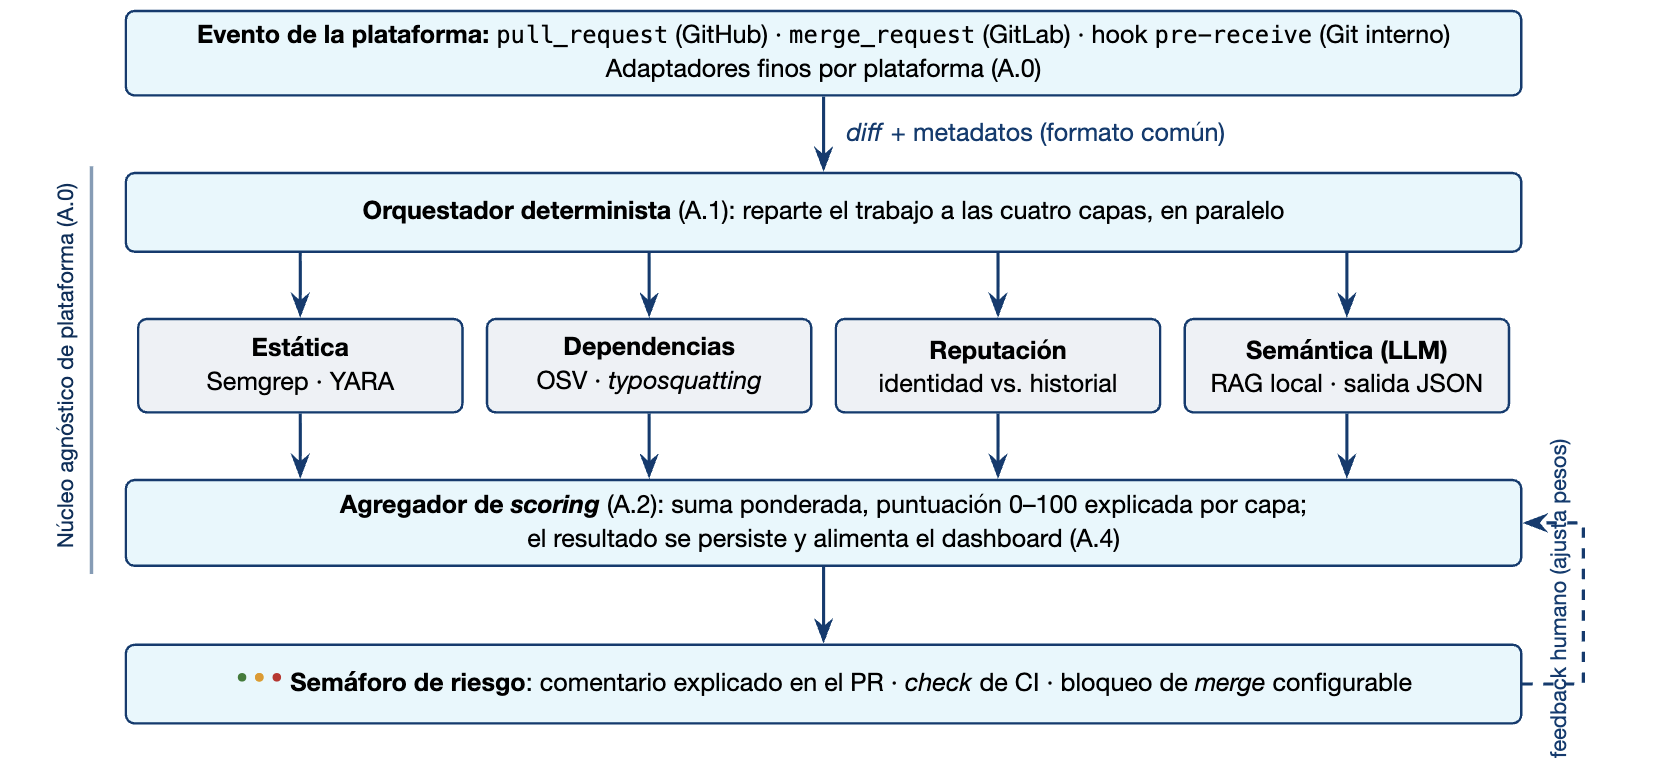
\includegraphics[width=0.82\textwidth]{diagrama_estructura.png}
\end{frame}

% ======================================================================
\begin{frame}[fragile]{04 \textperiodcentered\ El contrato entre capas}
\noindent{\large Interfaz única: mismo diff de entrada, mismo resultado de salida}\par\vspace{4pt}
{\color{inksoft}\footnotesize Cualquier capa nueva implementa esta interfaz y se registra por decorador; el orquestador nunca importa una capa concreta por nombre.}

\vspace{4pt}
\begin{columns}[T,onlytextwidth]
\begin{column}{0.52\textwidth}
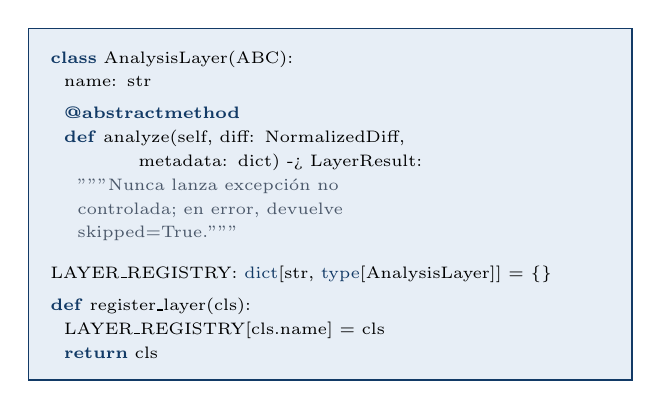
\begin{tikzpicture}
\node[card, text width=7.1cm, font=\MenloFont\fontsize{6.4}{8.6}\selectfont, align=left] {%
\textcolor{brandnavy2}{\textbf{class}} AnalysisLayer(ABC):\\
\ \ name: str\\[3pt]
\ \ \textcolor{brandnavy2}{\textbf{@abstractmethod}}\\
\ \ \textcolor{brandnavy2}{\textbf{def}} analyze(self, diff: NormalizedDiff,\\
\ \ \ \ \ \ \ \ \ \ \ \ \ metadata: dict) -\/> LayerResult:\\
\ \ \ \ \textcolor{inksoft}{"""Nunca lanza excepción no}\\
\ \ \ \ \textcolor{inksoft}{controlada; en error, devuelve}\\
\ \ \ \ \textcolor{inksoft}{skipped=True."""}\\[6pt]
LAYER\_REGISTRY: \textcolor{brandnavy2}{dict}[str, \textcolor{brandnavy2}{type}[AnalysisLayer]] = \{\}\\[3pt]
\textcolor{brandnavy2}{\textbf{def}} register\_layer(cls):\\
\ \ LAYER\_REGISTRY[cls.name] = cls\\
\ \ \textcolor{brandnavy2}{\textbf{return}} cls
};
\end{tikzpicture}
\end{column}
\begin{column}{0.44\textwidth}
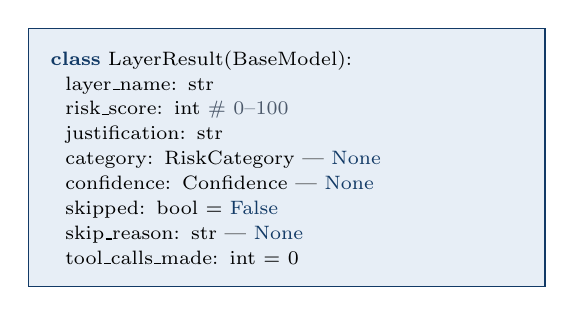
\begin{tikzpicture}
\node[card, text width=6.0cm, font=\MenloFont\fontsize{6.6}{9}\selectfont, align=left] {%
\textcolor{brandnavy2}{\textbf{class}} LayerResult(BaseModel):\\
\ \ layer\_name: str\\
\ \ risk\_score: int\ \textcolor{inksoft}{\# 0\textendash100}\\
\ \ justification: str\\
\ \ category: RiskCategory | \textcolor{brandnavy2}{None}\\
\ \ confidence: Confidence | \textcolor{brandnavy2}{None}\\
\ \ skipped: bool = \textcolor{brandnavy2}{False}\\
\ \ skip\_reason: str | \textcolor{brandnavy2}{None}\\
\ \ tool\_calls\_made: int = 0
};
\end{tikzpicture}

\vspace{3pt}
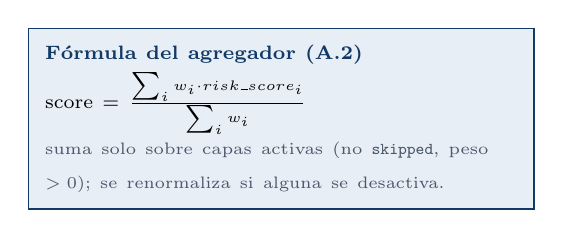
\begin{tikzpicture}
\node[card, text width=6.0cm, align=left, inner sep=6pt] {
  {\lbl\fontsize{7.4}{8}\selectfont Fórmula del agregador (A.2)}\\[2pt]
  {\MenloFont\fontsize{6.8}{8}\selectfont score = $\frac{\sum_i w_i \cdot \text{risk\_score}_i}{\sum_i w_i}$}\\[2pt]
  {\sub\fontsize{6.5}{7.4}\selectfont suma solo sobre capas activas (no \texttt{skipped}, peso $>0$); se renormaliza si alguna se desactiva.}
};
\end{tikzpicture}
\end{column}
\end{columns}
\end{frame}

% ======================================================================
\begin{frame}{05 \textperiodcentered\ Las cuatro capas}
\noindent{\large Cada capa es un módulo intercambiable}\par\vspace{4pt}
{\color{inksoft}\footnotesize Misma entrada (diff + metadata), misma salida (puntuación 0\textendash100 + justificación en texto). Se puede desactivar una capa por proyecto, o cambiar el proveedor de LLM, sin tocar el resto.}

\vspace{4pt}
\begin{columns}[T,onlytextwidth]
\begin{column}{0.5\textwidth}
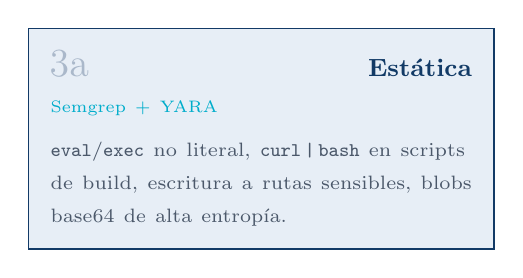
\begin{tikzpicture}
\node[card, text width=5.35cm] {
  {\MenloFont\fontsize{15}{15}\selectfont\color{linestrong} 3a}\hfill{\lbl\fontsize{9.5}{10.5}\selectfont Estática}\\[1pt]
  {\MenloFont\fontsize{6.4}{7}\selectfont\color{brandcyan} Semgrep + YARA}\\[4pt]
  {\sub\fontsize{7.2}{8.4}\selectfont \texttt{eval}/\texttt{exec} no literal, \texttt{curl\,|\,bash} en scripts de build, escritura a rutas sensibles, blobs base64 de alta entropía.}
};
\end{tikzpicture}

\vspace{6pt}
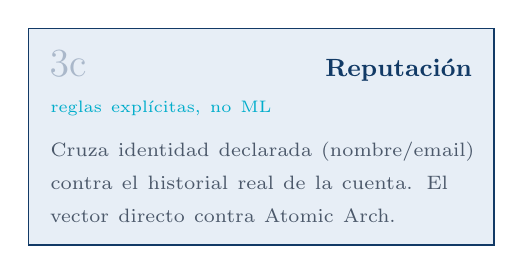
\begin{tikzpicture}
\node[card, text width=5.35cm] {
  {\MenloFont\fontsize{15}{15}\selectfont\color{linestrong} 3c}\hfill{\lbl\fontsize{9.5}{10.5}\selectfont Reputación}\\[1pt]
  {\MenloFont\fontsize{6.4}{7}\selectfont\color{brandcyan} reglas explícitas, no ML}\\[4pt]
  {\sub\fontsize{7.2}{8.4}\selectfont Cruza identidad declarada (nombre/email) contra el historial real de la cuenta. El vector directo contra Atomic Arch.}
};
\end{tikzpicture}
\end{column}
\begin{column}{0.5\textwidth}
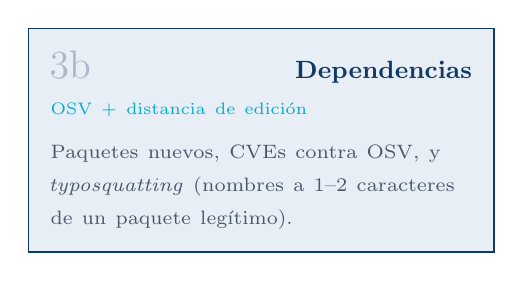
\begin{tikzpicture}
\node[card, text width=5.35cm] {
  {\MenloFont\fontsize{15}{15}\selectfont\color{linestrong} 3b}\hfill{\lbl\fontsize{9.5}{10.5}\selectfont Dependencias}\\[1pt]
  {\MenloFont\fontsize{6.4}{7}\selectfont\color{brandcyan} OSV + distancia de edición}\\[4pt]
  {\sub\fontsize{7.2}{8.4}\selectfont Paquetes nuevos, CVEs contra OSV, y \emph{typosquatting} (nombres a 1\textendash2 caracteres de un paquete legítimo).}
};
\end{tikzpicture}

\vspace{6pt}
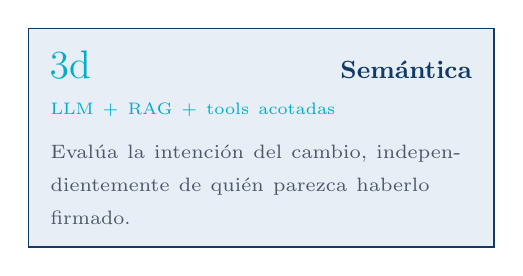
\begin{tikzpicture}
\node[cardcyan, text width=5.35cm] {
  {\MenloFont\fontsize{15}{15}\selectfont\color{brandcyan} 3d}\hfill{\lbl\fontsize{9.5}{10.5}\selectfont Semántica}\\[1pt]
  {\MenloFont\fontsize{6.4}{7}\selectfont\color{brandcyan} LLM + RAG + tools acotadas}\\[4pt]
  {\sub\fontsize{7.2}{8.4}\selectfont Evalúa la intención del cambio, independientemente de quién parezca haberlo firmado.}
};
\end{tikzpicture}
\end{column}
\end{columns}
\end{frame}

% ======================================================================
\begin{frame}{06 \textperiodcentered\ Formato de salida}
\centering
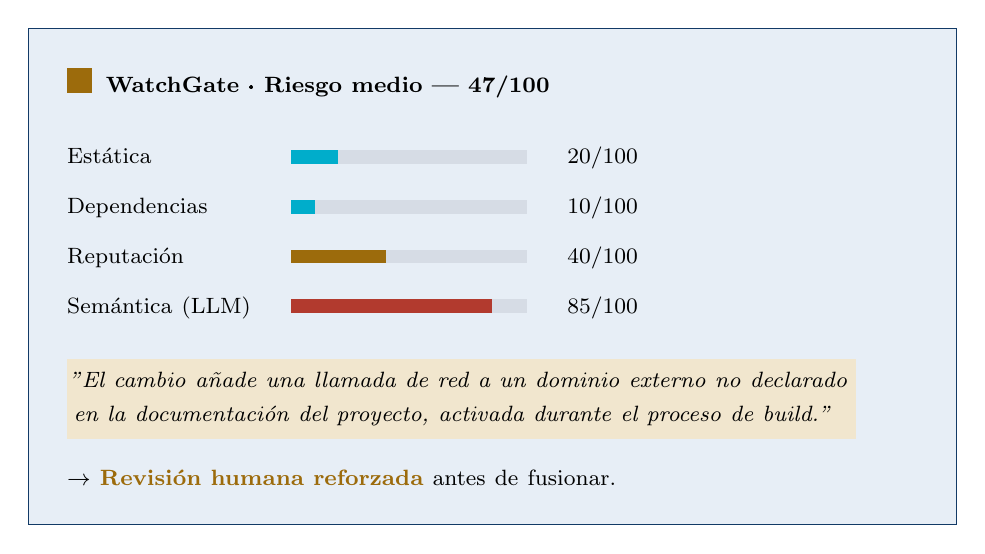
\begin{tikzpicture}
\node[card, text width=10.8cm, minimum height=6.3cm, inner sep=14pt] (t) {
  \begin{minipage}{10.4cm}
  {\MenloFont\fontsize{8.5}{10}\selectfont
  \textcolor{samber}{\rule{9pt}{9pt}}\hspace{5pt}\textbf{WatchGate \textperiodcentered\ Riesgo medio \textemdash\ 47/100}}

  \vspace{10pt}
  \renewcommand{\arraystretch}{1.5}
  \begin{tabular}{@{}l l r@{}}
  {\footnotesize Estática} & \tikz{\draw[linecol,line width=5pt] (0,0) -- (3,0); \draw[brandcyan,line width=5pt] (0,0) -- (0.6,0);} & {\MenloFont\footnotesize 20/100} \\
  {\footnotesize Dependencias} & \tikz{\draw[linecol,line width=5pt] (0,0) -- (3,0); \draw[brandcyan,line width=5pt] (0,0) -- (0.3,0);} & {\MenloFont\footnotesize 10/100} \\
  {\footnotesize Reputación} & \tikz{\draw[linecol,line width=5pt] (0,0) -- (3,0); \draw[samber,line width=5pt] (0,0) -- (1.2,0);} & {\MenloFont\footnotesize 40/100} \\
  {\footnotesize Semántica (LLM)} & \tikz{\draw[linecol,line width=5pt] (0,0) -- (3,0); \draw[semred,line width=5pt] (0,0) -- (2.55,0);} & {\MenloFont\footnotesize 85/100} \\
  \end{tabular}

  \vspace{10pt}
  \colorbox{sambersoft}{\begin{minipage}{9.8cm}\vspace{2pt}{\footnotesize\itshape "El cambio añade una llamada de red a un dominio externo no declarado en la documentación del proyecto, activada durante el proceso de build."}\vspace{2pt}\end{minipage}}

  \vspace{10pt}
  {\footnotesize $\rightarrow$ \textbf{\textcolor{samber}{Revisión humana reforzada}} antes de fusionar.}
  \end{minipage}
};
\end{tikzpicture}
\end{frame}

% ======================================================================
\begin{frame}{07 \textperiodcentered\ Capa estática}
\noindent{\large Patrones de código peligrosos conocidos}\par\vspace{4pt}
{\color{inksoft}\footnotesize Semgrep (reglas propias + registros públicos \texttt{p/security-audit}, \texttt{p/secrets}) sobre los hunks modificados, más YARA sobre el mismo contenido.}

\vspace{6pt}
\begin{columns}[T,onlytextwidth]
\begin{column}{0.52\textwidth}
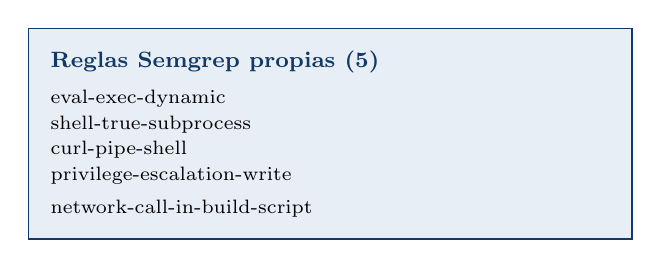
\begin{tikzpicture}
\node[card, text width=7.1cm, align=left] {
  {\lbl\fontsize{8}{8.8}\selectfont Reglas Semgrep propias (5)}\\[4pt]
  {\MenloFont\fontsize{6.6}{9.2}\selectfont
  eval-exec-dynamic\\
  shell-true-subprocess\\
  curl-pipe-shell\\
  privilege-escalation-write\\
  network-call-in-build-script}
};
\end{tikzpicture}
\end{column}
\begin{column}{0.44\textwidth}
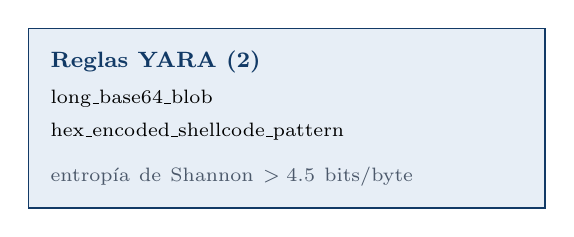
\begin{tikzpicture}
\node[card, text width=6.0cm, align=left] {
  {\lbl\fontsize{8}{8.8}\selectfont Reglas YARA (2)}\\[4pt]
  {\MenloFont\fontsize{6.6}{9.2}\selectfont
  long\_base64\_blob\\
  hex\_encoded\_shellcode\_pattern}\\[4pt]
  {\sub\fontsize{6.8}{8.4}\selectfont entropía de Shannon $>4.5$ bits/byte}
};
\end{tikzpicture}
\end{column}
\end{columns}

\vspace{8pt}
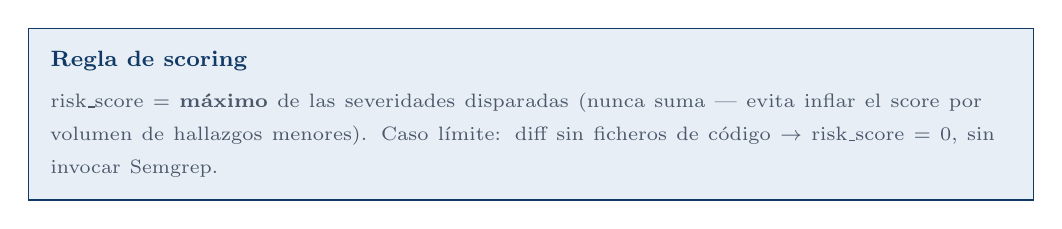
\begin{tikzpicture}
\node[cardcyan, text width=12.2cm, align=left] {
  {\lbl\fontsize{7.6}{8.4}\selectfont Regla de scoring}\\[3pt]
  {\sub\fontsize{7.2}{8.6}\selectfont risk\_score = \textbf{máximo} de las severidades disparadas (nunca suma \textemdash\ evita inflar el score por volumen de hallazgos menores). Caso límite: diff sin ficheros de código $\rightarrow$ risk\_score = 0, sin invocar Semgrep.}
};
\end{tikzpicture}
\end{frame}

% ======================================================================
\begin{frame}{08 \textperiodcentered\ Capa de dependencias}
\noindent{\large Paquetes nuevos, CVEs conocidas y \emph{typosquatting}}\par\vspace{4pt}
{\color{inksoft}\footnotesize Solo se activa si el diff toca un manifiesto: \texttt{package.json}, \texttt{requirements.txt}, \texttt{Pipfile}, \texttt{PKGBUILD}, \texttt{Cargo.toml}.}

\vspace{8pt}
\begin{tikzpicture}
\node[card, text width=12.2cm, align=left] (osv) {
  {\lbl\fontsize{7.8}{8.6}\selectfont Consulta OSV}\\[2pt]
  {\sub\fontsize{7.2}{8.4}\selectfont \texttt{POST api.osv.dev/v1/query} por cada dependencia nueva o con versión cambiada; caché SQLite local con TTL de 24h.}
};
\node[card, below=6pt of osv, text width=12.2cm, align=left] (typo) {
  {\lbl\fontsize{7.8}{8.6}\selectfont Typosquatting}\\[2pt]
  {\sub\fontsize{7.2}{8.4}\selectfont distancia de Levenshtein $\leq 2$ contra el top-N de paquetes por descargas de ese ecosistema (p.\ ej.\ \texttt{"1odash"} vs.\ \texttt{"lodash"}).}
};
\node[cardcyan, below=6pt of typo, text width=12.2cm, align=left] (score) {
  {\lbl\fontsize{7.8}{8.6}\selectfont Scoring (máximo entre señales)}\\[2pt]
  {\sub\fontsize{7.2}{8.4}\selectfont CVE crítica/alta $\rightarrow$ 90 \textperiodcentered\ typosquatting probable $\rightarrow$ 75 \textperiodcentered\ script de instalación con hallazgos de red/ejecución $\rightarrow$ 80. Caso límite: fallo de red a OSV \textbf{no} sube el score, se anota como "no verificable".}
};
\end{tikzpicture}
\end{frame}

% ======================================================================
\begin{frame}{09 \textperiodcentered\ Capa de reputación}
\noindent{\large Identidad declarada frente a historial real de la cuenta}\par\vspace{4pt}
{\color{inksoft}\footnotesize Reglas explícitas, no ML. Nunca hace llamadas HTTP: toda la metadata llega ya resuelta desde el adaptador de plataforma.}

\vspace{8pt}
\centering
{\small
\renewcommand{\arraystretch}{1.4}
\begin{tabular}{@{}l r@{}}
\toprule
\textbf{\footnotesize Señal} & \textbf{\footnotesize Puntos} \\
\midrule
Cuenta con menos de 30 días de antigüedad & +30 \\
Cero contribuciones previas al repositorio & +20 \\
Email del commit no verificado por la plataforma & +25 \\
Repo firma habitualmente, este commit no está firmado & +30 \\
Firmado, pero con clave nunca vista para ese login & +40 \\
\bottomrule
\end{tabular}
}

\vspace{10pt}
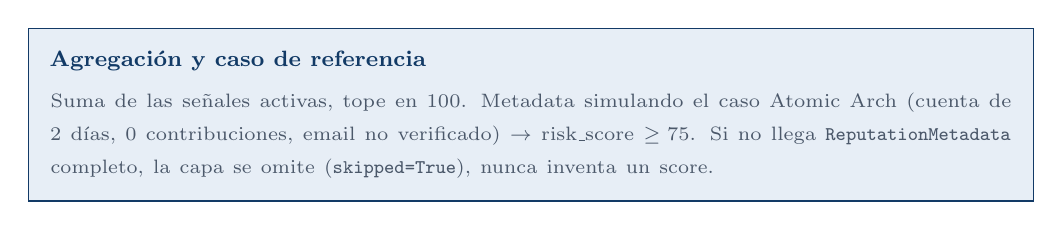
\begin{tikzpicture}
\node[cardcyan, text width=12.2cm, align=left] {
  {\lbl\fontsize{7.8}{8.6}\selectfont Agregación y caso de referencia}\\[3pt]
  {\sub\fontsize{7.2}{8.4}\selectfont Suma de las señales activas, tope en 100. Metadata simulando el caso Atomic Arch (cuenta de 2 días, 0 contribuciones, email no verificado) $\rightarrow$ risk\_score $\geq 75$. Si no llega \texttt{ReputationMetadata} completo, la capa se omite (\texttt{skipped=True}), nunca inventa un score.}
};
\end{tikzpicture}
\end{frame}

% ======================================================================
\begin{frame}{10 \textperiodcentered\ Capa semántica}
\noindent{\large La evaluación no se basa únicamente en el contenido visible del diff}\par\vspace{4pt}
{\color{inksoft}\footnotesize Antes de preguntar, el sistema ya le sirve contexto de casos reales parecidos (RAG). Durante el análisis, el modelo puede pedir investigar más por su cuenta \textemdash\ hasta un límite duro.}

\vspace{2pt}
\centering
\scalebox{0.90}{%
\begin{tikzpicture}
\node[card, text width=12.2cm, align=left, inner sep=6pt] (s1) {\lbl\fontsize{8}{8.6}\selectfont 01\hspace{6pt} Control de coste\\ \sub\fontsize{7.2}{8.2}\selectfont ¿Hay presupuesto de tokens este mes? ¿Este diff exacto ya se analizó? Si no hay presupuesto, se omite sin llamar al LLM.};
\node[card, below=4pt of s1, text width=12.2cm, align=left, inner sep=6pt] (s2) {\lbl\fontsize{8}{8.6}\selectfont 02\hspace{6pt} RAG \textemdash\ recuperación automática\\ \sub\fontsize{7.2}{8.2}\selectfont El propio sistema resume el diff y busca los 3 casos más parecidos en un corpus local (XZ Utils, Atomic Arch, prt-scan, MITRE ATT\&CK). El LLM no lo pide: ya le llega servido.};
\node[cardcyan, below=4pt of s2, text width=12.2cm, align=left, inner sep=6pt] (s3) {\lbl\fontsize{8}{8.6}\selectfont 03\hspace{6pt} El LLM investiga \emph{(si lo necesita)}\\ \sub\fontsize{7.2}{8.2}\selectfont En este paso el modelo decide si necesita más contexto: puede invocar hasta 3 herramientas antes de responder.\\[2pt] {\MenloFont\fontsize{6.6}{7}\selectfont\color{brandnavy2} lookup\_package\_registry \textperiodcentered\ get\_commit\_history \textperiodcentered\ fetch\_referenced\_file}};
\node[card, below=4pt of s3, text width=12.2cm, align=left, inner sep=6pt] (s4) {\lbl\fontsize{8}{8.6}\selectfont 04\hspace{6pt} Salida estructurada\\ \sub\fontsize{7.2}{8.2}\selectfont {\MenloFont\fontsize{7}{7.6}\selectfont risk\_score \textperiodcentered\ category \textperiodcentered\ justification \textperiodcentered\ confidence} \textemdash\ JSON validado, se cachea, se combina con las otras 3 capas.};
\end{tikzpicture}%
}
\end{frame}

% ======================================================================
\begin{frame}{11 \textperiodcentered\ Infraestructura necesaria}
\noindent{\large Tenemos acceso a Google Cloud Platform}\par\vspace{4pt}
{\color{inksoft}\footnotesize No tenemos experiencia previa con GCP: esto es lo que creemos que vamos a necesitar, a falta de validarlo según avance el proyecto \textemdash\ no una arquitectura cerrada.}

\vspace{1pt}
\centering
{\fontsize{7.3}{8.7}\selectfont
\renewcommand{\arraystretch}{1.15}
\begin{tabular}{@{}p{2.35cm} p{9.5cm}@{}}
\toprule
\textbf{\footnotesize Servicio} & \textbf{\footnotesize Para qué lo necesitamos} \\
\midrule
\textbf{Cloud SQL (Postgres + pgvector)} & Sustituye el SQLite del dashboard \emph{y} guarda los embeddings del corpus RAG en la misma base de datos (extensión \texttt{pgvector}), en vez de montar un servicio de vectores aparte. \\
\textbf{Cloud Run} & Backend del dashboard (FastAPI) sin gestionar servidores; escala a cero entre análisis. \\
\textbf{Secret Manager} & El backend en Cloud Run necesita el secreto OAuth de GitHub y la contraseña de Cloud SQL; viven aquí cifrados, no en variables de entorno en claro. \\
\textbf{Cloud Logging} & Ingesta del logging JSON estructurado que ya exige el núcleo (A.0). \\
\textbf{Vertex AI (Gemini)} & Proveedor de LLM alternativo a Anthropic para la capa semántica (\texttt{LLMClient} ya es sustituible). \\
\textbf{Identity Platform} & Que un cliente empresarial inicie sesión con su propio proveedor de identidad (Okta, Azure AD\ldots) en vez de una cuenta de GitHub, sin programar cada federación a mano. \\
\bottomrule
\end{tabular}
}
\end{frame}

\end{document}
